% Chapter 3
\chapter{Calibration System for RGBD Cameras} % Main chapter title
\label{sens_CalibrationSystem} % For referencing the chapter elsewhere, use \ref{sens_CalibrationSystem} 
%
%
\section{Rail System}%
As already shown in chapter \ref{sens_introduction} figure \ref{trackingModuleOnKinectV2CalibrationSystem}, the whole calibration system consists of an RGB-D camera, a plane of round dot pattern, rail, and a BLE Optical-Flow tracking module. 
Other than the round dot pattern standing in front of the 3D camera for offering distortion information, all of the rest parts of the whole calibration system are centered on the rail, which is made with 80/20s. Taking the round dot pattern plane as plane \(X^wY^w\), the rail is placed right perpendicular to the dot pattern along the direction of \(Z^w\) axis. Both of the RGB-D camera and the BLE Optical-Flow tracking module are mounted on the slider of the rail. \par
%
Sitting on the top of the elevated carriage of the slider, the RGB-D camera's vision keeps being horizontal, parallel with \(Z^w\) axis. And the origin is chosen right at the center of the camera's field of view, like figure \ref{cameraFieldOfView} shows.\par
%
\begin{figure}[h]
\centering
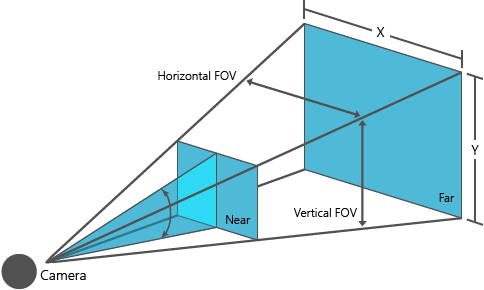
\includegraphics[width=\textwidth]{cameraFieldOfView}
\caption{World Coordinate Frame}
\label{cameraFieldOfView}
\end{figure}%
%
The BLE Optical-Flow tracking module is mounted at the bottom of the rail to tracking the movements of the slider, as shown in figure \ref{MountedTrackingModuleObservingRail}. With infrared LED projecting injective rays onto the inner surface of the 80/20 groove, Optical-Flow sensor could generate accumulated X/Y value based on its observed optical flow changes (the changes of diffuse reflection rays from inner surface, generated by LED). The white re-stickable strip covering on the joint between PCB and OF sensor is for shocking absorption. Sliding along the rail, the accumulated Y value is always zero, and the accumulated X value records the movements of the slider, and will be sent into PC over the air by the BLE module. 
%
\par
%
\begin{figure}[h]
\centering
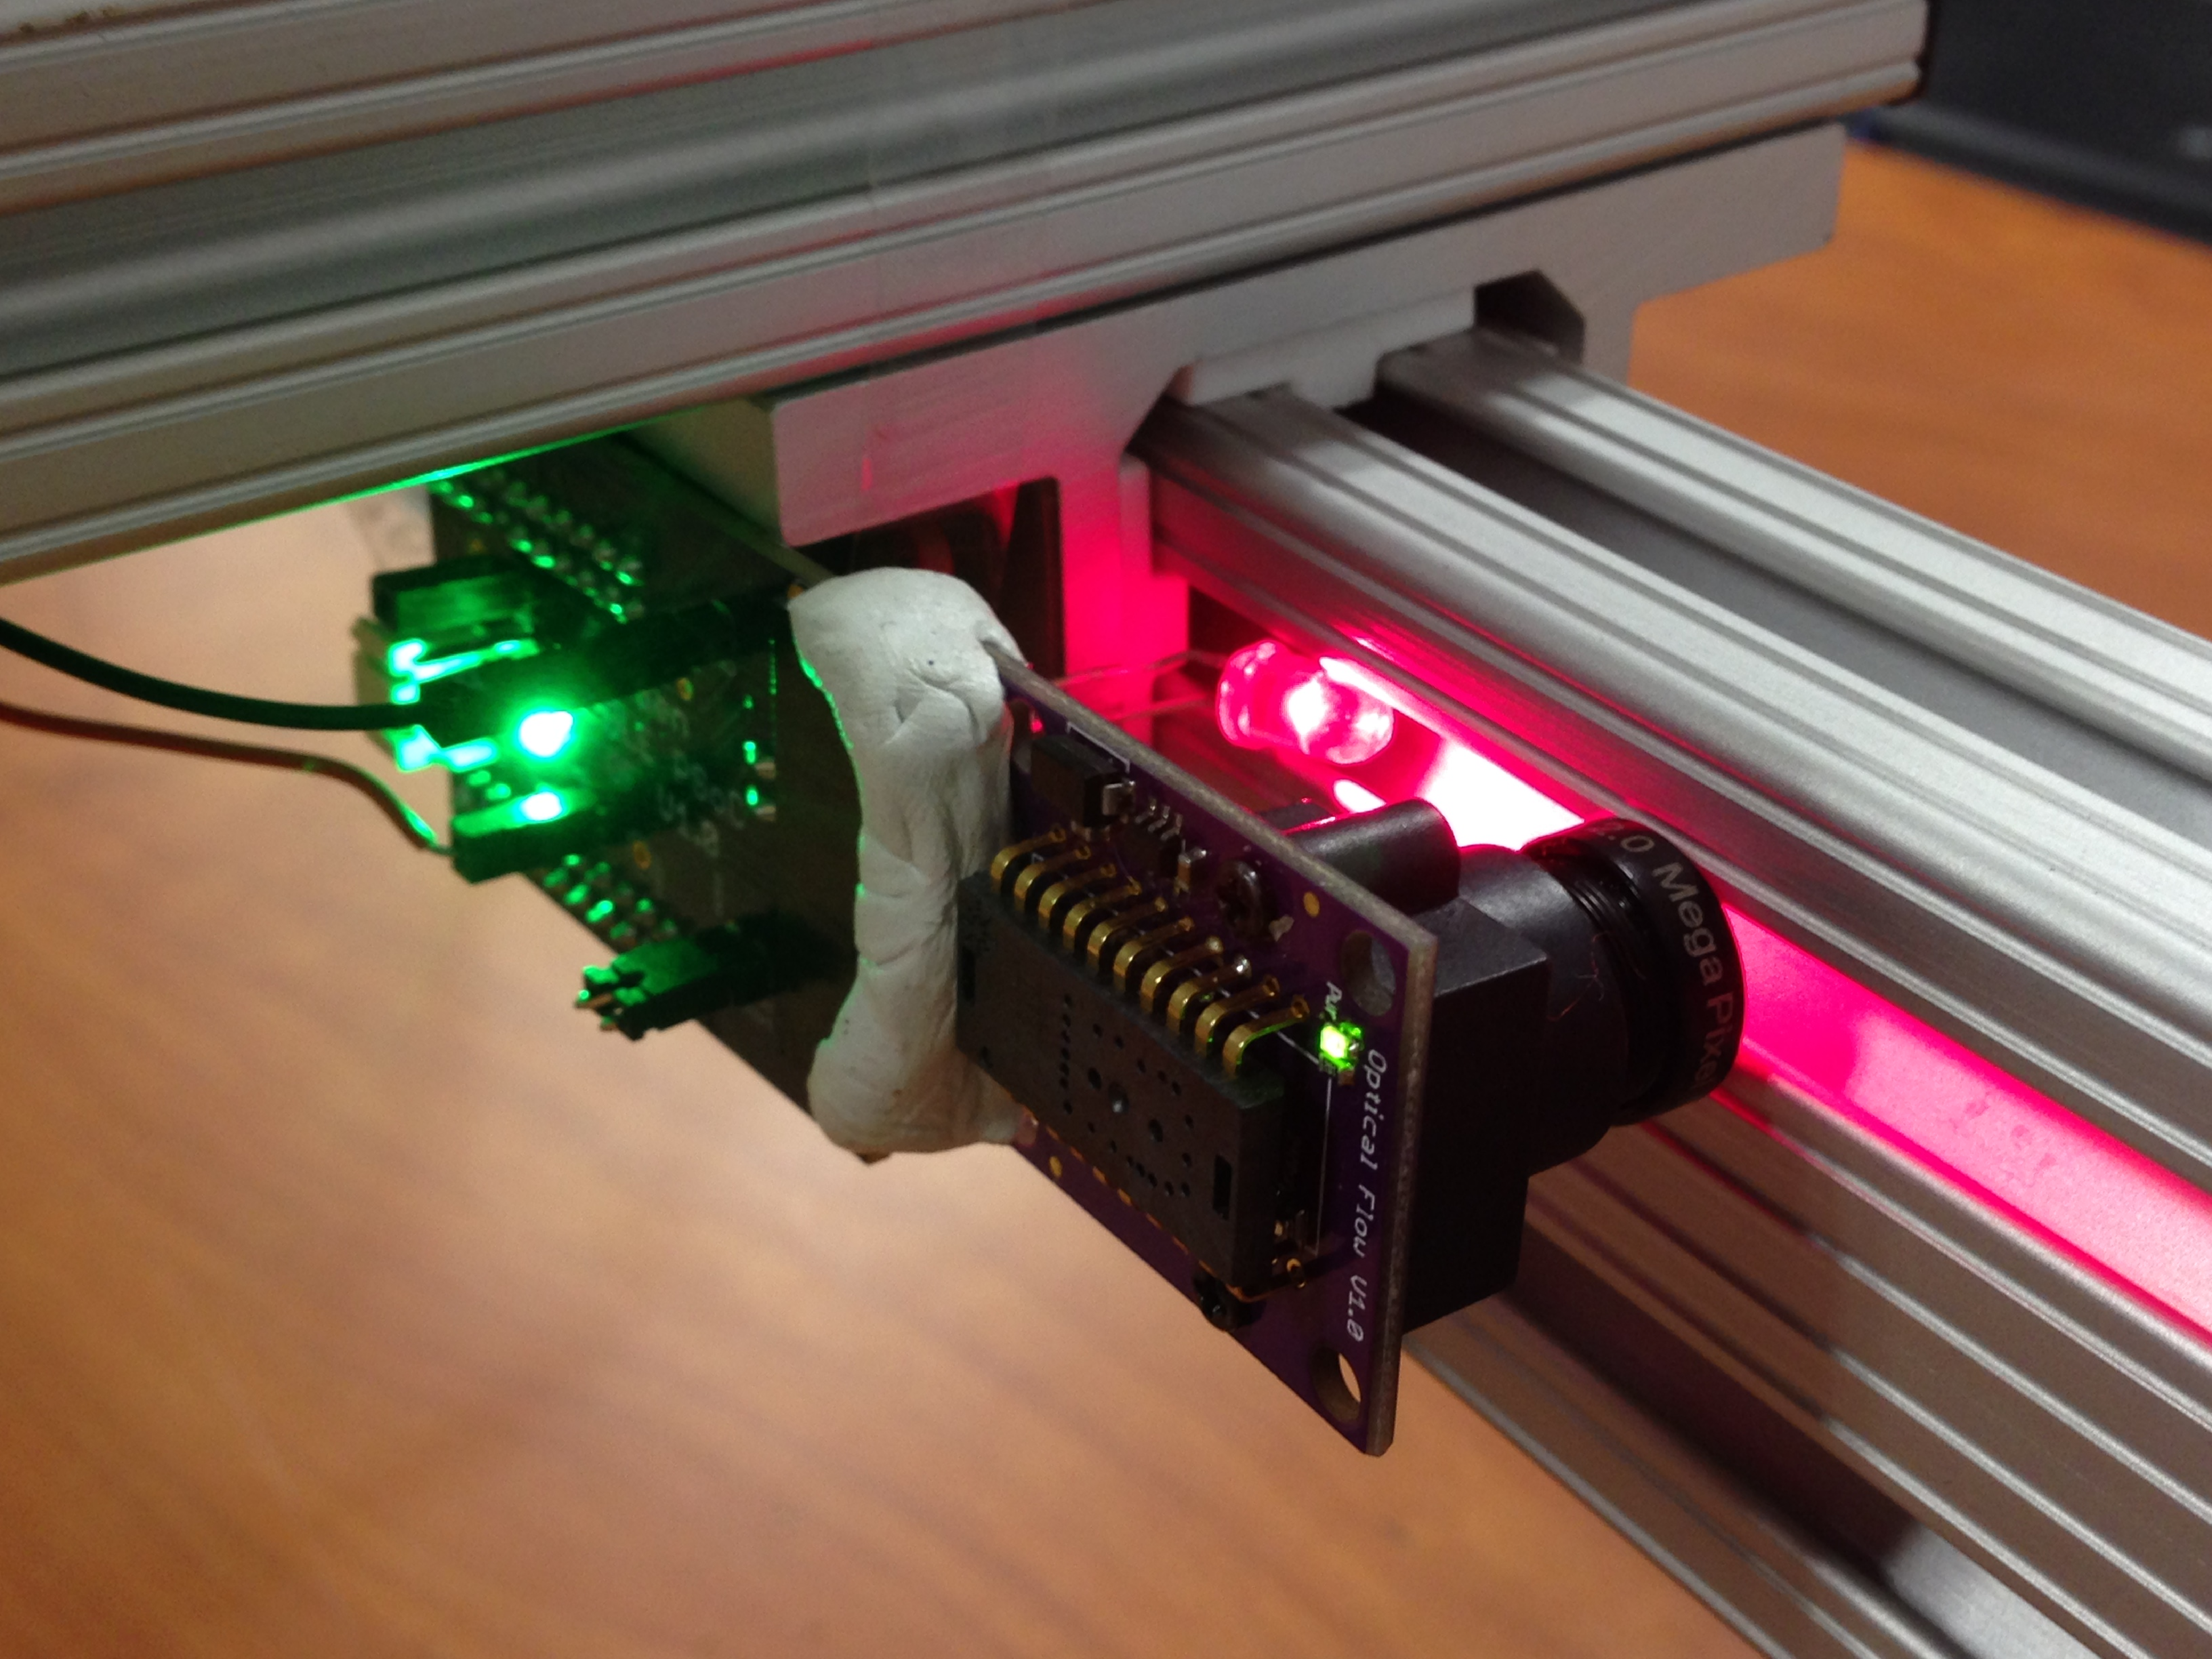
\includegraphics[width=0.85\textwidth]{MountedTrackingModuleObservingRail}
\caption{Mounted BLE Optical-Flow Tracking Module}
\label{MountedTrackingModuleObservingRail}
\end{figure}%
%
%
\section{Optical-Flow Sensor for Z Tracking}
%
%
%
%
\section{Bluetooth Low Energy for wireless communication}
%
%
%
%
%
%
%
Chapter 4: results for 3 types of RGB-D cameras.\\
Chapter 5: conclusion\\





































